\documentclass[a4paper, oneside, openany, dvipsnames, table, 12pt]{article}
\usepackage[italian,british]{babel}
\usepackage{../../../Template/AFKstyleEng}
\usepackage{hyperref}
\usepackage{amsmath}
\usepackage{verbatim}
\newcommand{\Titolo}{Developer Manual}

\newcommand{\Gruppo}{TeamAFK}

\newcommand{\Redattori}{Simone Federico Bergamin \newline Olivier Utshudi}

\newcommand{\Verificatori}{}

\newcommand{\pathimg}{../Developer_manual/img/logoAFK.png}

\newcommand{\Approvatore}{}

\newcommand{\Distribuzione}{Prof. Vardanega Tullio \newline Prof. Cardin Riccardo \newline TeamAFK}

\newcommand{\Uso}{External}

\newcommand{\NomeProgetto}{Predire in Grafana}

\newcommand{\Mail}{gruppoafk15@gmail.com}

\newcommand{\Versionedoc}{1.0.0}

\newcommand{\DescrizioneDoc}{Developer manual made by \textit{TeamAFK} for the project \textit{Predire in Grafana}.}

\makeindex

\begin{document}
\frontispiece{}

%------------------ COLORI TABELLE 
\definecolor{pari}{RGB}{255, 207, 158} %{HTML}{E1F5FE} %azzurrino
\definecolor{dispari}{HTML}{FAFAFA} %bianco/grigetto 

%definizione colori per tabelle (tranne copertina)
\definecolor{redafk}{RGB}{255, 133, 51}
\definecolor{grey2}{RGB}{204, 204, 204}
\definecolor{greyRowafk}{RGB}{234, 234, 234}
\definecolor{lastrowcolor}{RGB}{176, 196, 222} %steel blue %{255,165,0} orange %{RGB}{255, 207, 158}
\rowcolors{2}{pari}{dispari}
\renewcommand{\arraystretch}{1.5}

%------------------

%------------------ PER SISTEMARE INDICE TABELLE E FIGURE 
\makeatletter
\renewcommand*\l@figure{\@dottedtocline{1}{1.5em}{3em}}% 3em instead of 2.3em
\let\l@table\l@figure
\makeatother
%------------------

\newpage
\section*{Changelog}
\begin{longtable}{c c C{3.5cm} C{4cm} C{3cm}}
		\rowcolor{redafk}
\textcolor{white}{\textbf{Version}} & 
\textcolor{white}{\textbf{Date}} & 
\textcolor{white}{\textbf{Description}} & 
\textcolor{white}{\textbf{Name}} & 
\textcolor{white}{\textbf{Role}}\\
		\endfirsthead
		\rowcolor{redafk}
\textcolor{white}{\textbf{Version}} & 
\textcolor{white}{\textbf{Date}} & 
\textcolor{white}{\textbf{Description}} & 
\textcolor{white}{\textbf{Name}} & 
\textcolor{white}{\textbf{Role}}\\
		\endhead
		1.0.0 & 2020-06-10 & Document approved for RQ & Olivier Utshudi & \textit{Manager}\\
		0.7.0 & 2020-06-04 & Writed and checked section \S 7 - \S A & Davide Zilio \newline Fouad Farid & \textit{Programmer} \newline \textit{Verifier} \\
		0.6.0 & 2020-06-04 & Writed and checked section \S 6  & Simone Federio Bergamin \newline Fouad Farid & \textit{Programmer} \newline \textit{Verifier} \\
		0.4.0 & 2020-06-04 & Writed and checked section \S 5 & Olivier Utshudi \newline Simone Meneghin & \textit{Programmer} \newline \textit{Verifier} \\
		0.3.0 & 2020-06-04 & Writed and checked section \S 4 & Simone Federico Bergamin \newline Simone Meneghin & \textit{Programmer}\newline \textit{Verifier}\\
		0.2.0 & 2020-06-03 & Writed and checked sections \S 2- \S 3 & Olivier Utshudi \newline Simone Meneghin & \textit{Programmer}\newline \textit{Verifier}\\
		0.1.0 & 2020-06-03 & Writed and checked section \S 1 & Simone Federico Bergamin \newline Fouad Farid & \textit{Programmer}\newline \textit{Verifier}
	\end{longtable}

%Didascalia tabelle/immagini (prendono come riferimento la subsection)
\counterwithin{table}{subsection}
\counterwithin{figure}{subsection}
\newpage

%indice, indice figure e indice tabelle
\tableofcontents
\newpage
\listoffigures
\newpage
%\listoftables
\newpage

\section{Introduction}
	\subsection{Document's purpose}
	Il manuale dello sviluppatore permette ad ogni sviluppatore che si approcci al prodotto software \emph{"Predire in Grafana"} di assimilare le informazioni principali per poter manutenere e estendere tale prodotto. All'interno del documento verrà descritto il prodotto in modo dettagliato, consentendo allo sviluppatore di ottenere una spiegazione esaustiva necessaria per l'attività che andrà a svolgere.

The developer's manual allows each developer reader to absorb \emph{"Predire in Grafana"}'s product key information to maintain and extend the product itself.
This document describes the product in its totality, giving the developer an exaustive explanation required for his tasks.
	
\subsection{Predire in Grafana’s Purpose}

\emph{"Predire in Grafana"} è un plugin realizzato per la piattaforma open source\glo Grafana che permette di calcolare delle previsioni su un flusso dati. Viene utilizzato un algoritmo addestrato dall'utente, la cui definizione è contenuta in un file in formato JSON\glo, per poter effettuare le previsioni.  Viene fornito un applicativo esterno per l'addestramento degli algoritmi di previsione, attualmente sono implementati gli algoritmi di Support Vector Machine\glo e Regressione Lineare\glo . Nello specifico il plugin monitora i dati in ingresso da un certo flusso, come
per esempio percentuali di utilizzo della memoria o temperatura del processore, e produce delle previsioni che vengono successivamente mostrate attraverso l'interfaccia graficaG di Grafana. Il plugin rimane in esecuzione e riceve continuamente informazioni in ingresso da un flusso di dati. In questo modo gli operatori potranno monitorare eventuali cambiamenti sul flusso dati grazie alla previsione in real time\glo ed intervenire, se necessario, sull'origine del problema. 
 
\emph{"Predire in Grafana"} is a plugin made for Grafana which is an open source\glo platform commonly used to analyze data series. The plugin allows users to predict datas on a stream data. \emph{"Predire in Grafana"} plugin uses a JSON file which contains a trained algorithm definition to get predictions. Users can use an external training tool, which use Machine Learning\glo , to get these JSON' files. At the moment only Support Vector Machine and Linear Regression algorithm are implemented. In more detail input datas, like cpu's usage and cpu's temperature, are constantly monitored to get predictions on the aspect you want to examine. Predictions are shown throght Grafana GUI and continue to be updated after being calculated from datas coming from a database. Thanks to this operators can monitor each process and intervene at the root of the problem whenever neccessary.


\subsection{Glossary}
A fine documento viene riportato nell'appendice un glossario che racchiude al suo interno ciascun termine che necessita di una spiegazione dettagliata per risultare più comprensibile al lettore. Tali termini vengono contrassegnati nel documento con una G a pedice.
 
At the end of the document in the appendix is available a glossary where explanations for new or ambiguous terms can be found. These are marked with a subscript G.

\subsection{References}
\subsubsection{Installation}
\begin{itemize}
	\item \url{https://nodejs.org/en/} (\url{https://nodejs.org/it/});
	\item \url{https://git-scm.com/};
	\item \url{https://www.gitkraken.com/};
	\item \url{https://grafana.com/get};
	\item \url{https://www.jetbrains.com/idea/}.
\end{itemize}
\subsubsection{Technologies}
\begin{itemize}
	\item \url{https://reactjs.org/docs/getting-started.html};
	\item \url{https://grafana.com/docs/grafana/latest/developers/plugins/};
	\item \url{https://www.jetbrains.com/help/idea/eslint.html}.
\end{itemize}
\subsubsection{Legal}
\begin{itemize}
	\item \url{https://www.apache.org/licenses/LICENSE-2.0}.
\end{itemize}

\subsubsection{Informative}
\begin{itemize}
	\item \url{https://en.wikipedia.org/wiki/Linear_regression};
	\item \url{https://en.wikipedia.org/wiki/Support_vector_machine}.
\end{itemize}
	


\pagebreak
\section{System Requirements}
Here the requirements for use of the product are listed.

\subsection{Minimum Hardware Requirements}
Here the requirements for use of the product are listed.
\begin{itemize}
	\item 2GB of RAM;
	\item 5GB of space on a drive;
	\item Dual core processor.	
\end{itemize}

\subsection{Compatible Operating Systems}
The software was developed and tested on the following:
\begin{itemize}
	\item Windows 10;
	\item MacOS 10.15;
	\item Ubuntu 18, 20.
\end{itemize}

\subsection{Compatible Browsers}
Predire in Grafana can be accessed through the following browsers:
\begin{itemize}
	\item Google Chrome version 58 or newer;
	\item Mozilla Firefox version 54 or newer;
	\item Apple Safari version 10 or newer;
	\item Microsoft Edge version 14 or newer;
	\item Opera version 55 or newer.
\end{itemize}




\pagebreak
\section{The training tool}
Here the appropriate way of using the training tool is explained in detail.

\subsection{Access}
The tool is a dynamic web page and can thus be accessed via browser.

\subsection{Uploading a CSV file in the tool}
The user will need to feed the tool a CSV file containing properly marked values for the algorithm the user has intention of training.

This can be done by selecting the "Select file" button, which will open a window from which the user will be able to select the CSV file he has intention of uploading.

\begin{figure}[H]
\centering
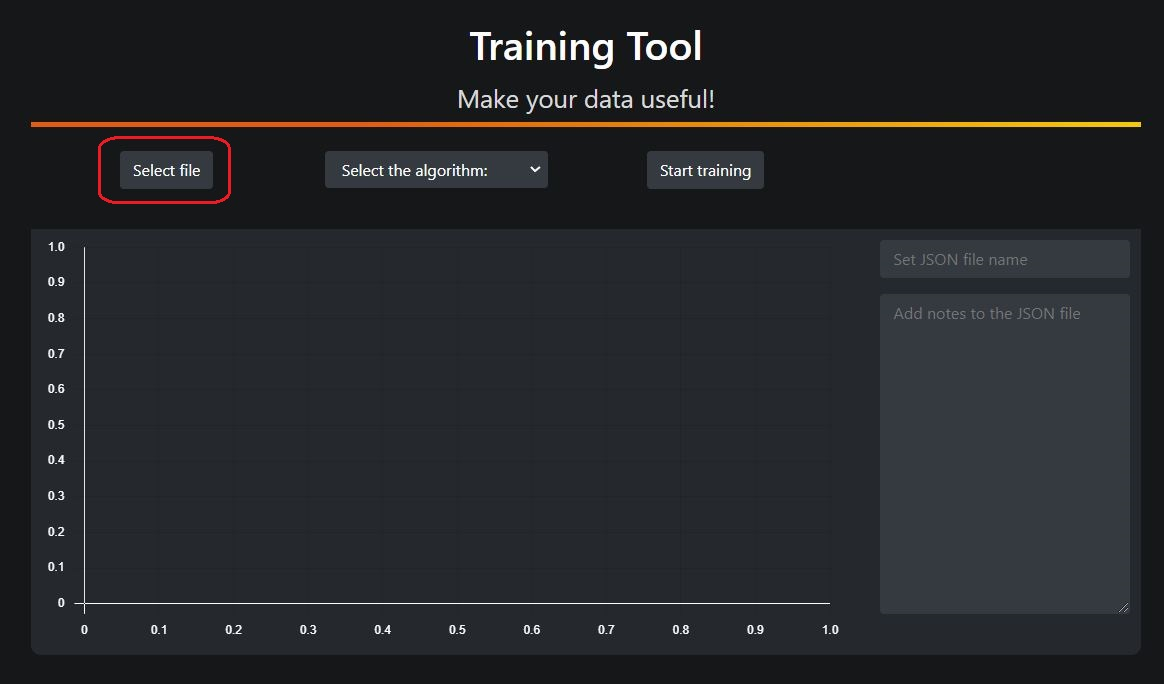
\includegraphics[scale=0.65]{img/tool/screen_1_tool.JPG}
\caption{CSV-File selector}
\end{figure}
\newpage

\subsection{Selection of the algorithm}
The user will have to choose between training a Support Vector Machine or a Linear Regression algorithm with the CSV file he has given to the tool.

To do this, the user can open a drop-down menu called "Select the algorithm" which displays the two algorithms that can be chosen. The preferred algorithm can at this point be selected.
\begin{figure}[H]
\centering
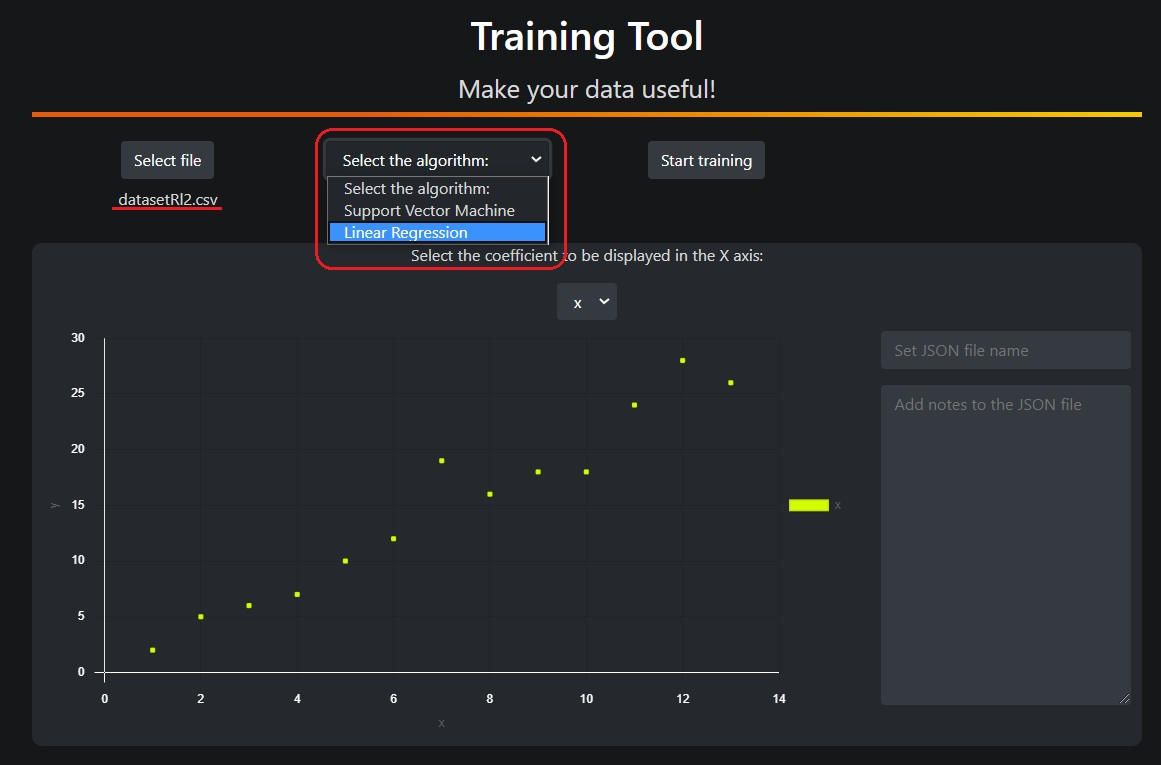
\includegraphics[scale=0.65]{img/tool/screen_2_tool.JPG}
\caption{Training algorithm selector}
\end{figure}
Should the user have uploaded training data incompatible with the selected algorithm, an error message will be displayed on selection of the "Start training" button.\newline
\begin{figure}[H]
\centering
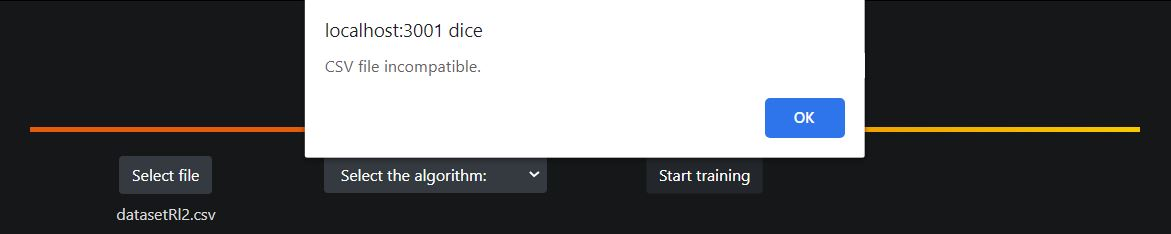
\includegraphics[scale=0.65]{img/tool/error_alg.JPG}
\caption{Incompatible algorithm uploaded}
\end{figure}
\newpage
\subsection{Training operation}
The tool will now be able to perform the training operation by simply  having the user select the “Start training” button. The tool will now have produced a JSON file containing the values needed for use in the plug-in.
\begin{figure}[H]
\centering
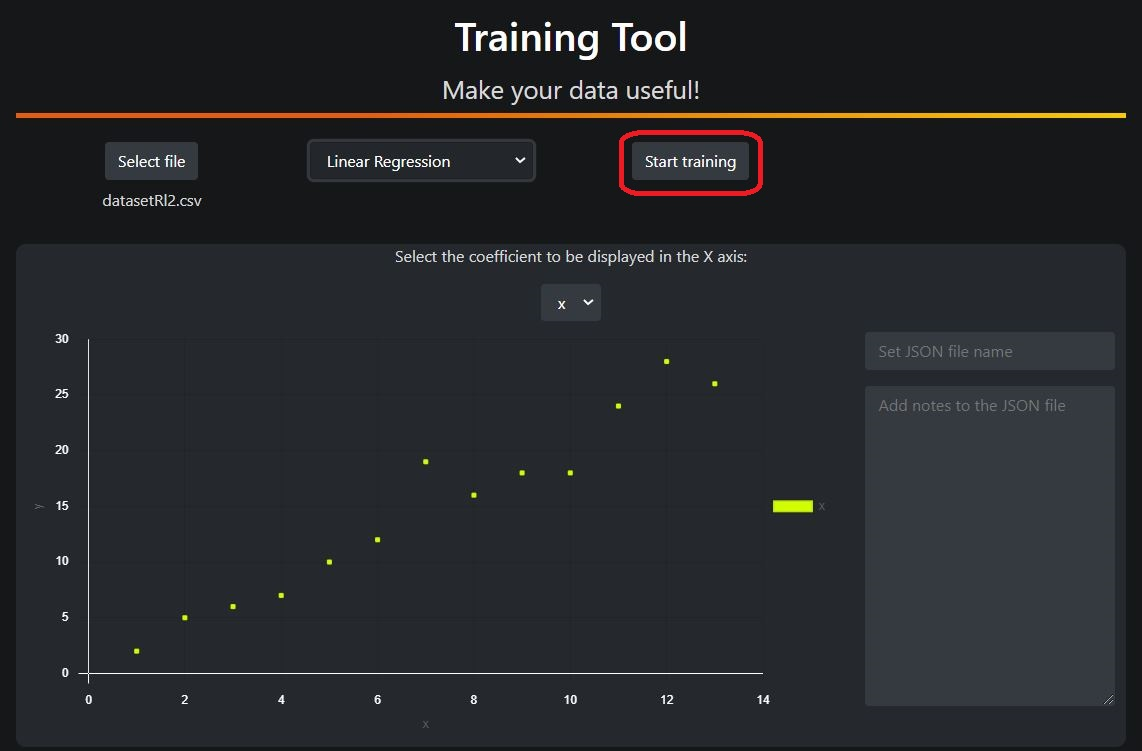
\includegraphics[scale=0.65]{img/tool/screen_3_1_tool.JPG}
\caption{Training operation with graphic point}
\end{figure}

A message will be displayed on selection of the "Start training" button if the training operation is successfully completed.
\newline
\begin{figure}[H]
\centering

\includegraphics[scale=0.65]{img/tool/screen_4_1_tool.JPG}
\caption{Training operation is successfully completed}
\end{figure}  
\newpage
\subsection{Obtaining the JSON file}
The user can now select the “Download” button, which will only appear once the training operation has ended succesfully, and receive the JSON file.
\begin{figure}[H]
\centering
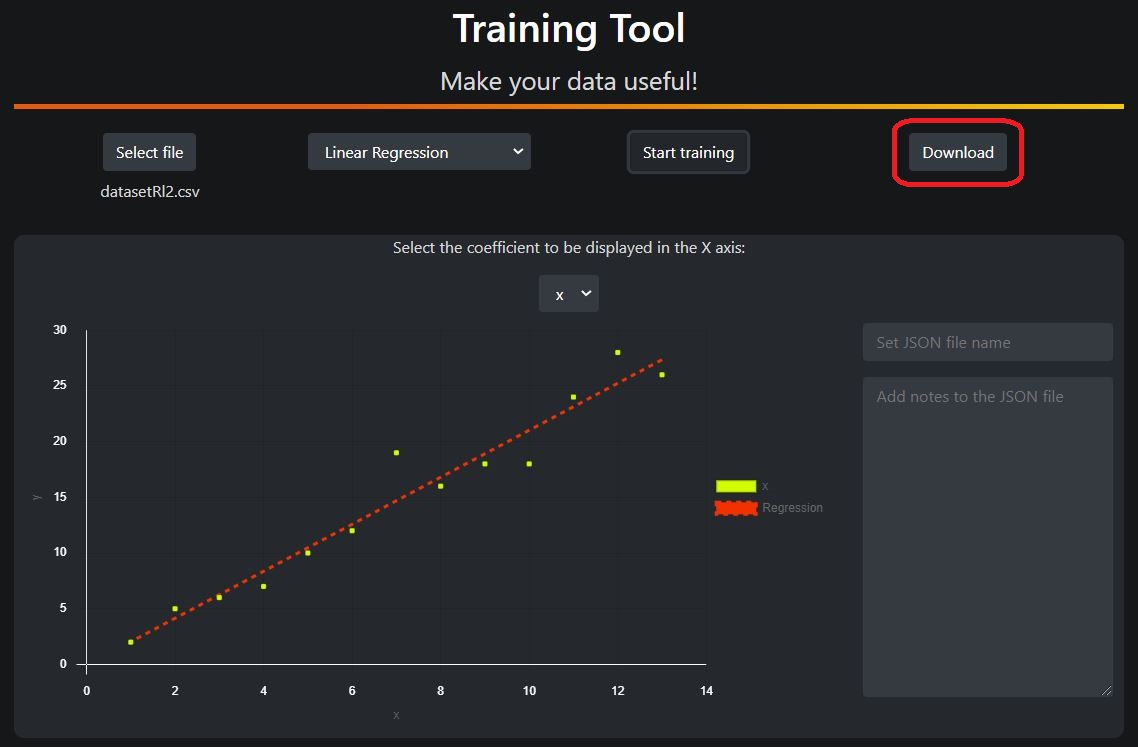
\includegraphics[scale=0.65]{img/tool/tool_5_1_tool.JPG}
\caption{The "Download" button is then clickable}
\end{figure} 
\newpage
\subsection{Info point}
Additional information can be accessed by selecting the "information" button, once selected a step-by-step guide will appear.

\begin{figure}[H]
\centering

\includegraphics[scale=0.65]{img/tool/screen_info_tool_2.JPG}
\caption{Info point button}
\end{figure} 

\subsubsection{Bug reporting}
The email address to which bug reports should be sent is displayed below the step-by-step guide, we will later explain in greater detail how to report a bug.


\pagebreak
\section{The plug-in}
Here a step by step explanation will guide the user through the proper usage of the prediction plug-in.

\subsection{Loading the plug-in}
\begin{enumerate}
	\item the user will have to select the plus icon from the sidebar, from which a drop-down menu containing three options will appear; from this menu the "dashboard" option has to be selected;


\begin{figure}[H]
\centering
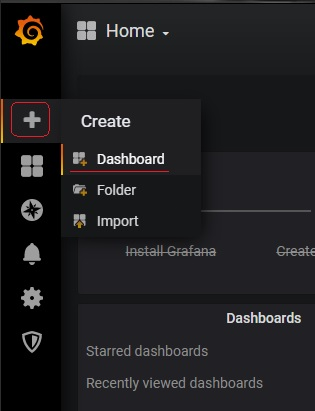
\includegraphics[scale=0.90]{img/plug-in/plus_dash.png}
\caption{Training operation with graphic point}
\end{figure}


	\item the user will now have to select the "Chose Visualization" button;


\begin{figure}[H]
\centering
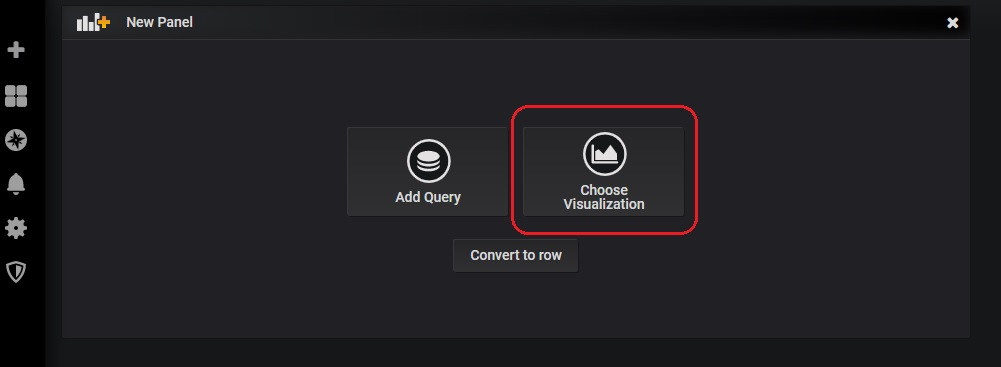
\includegraphics[scale=0.65]{img/plug-in/visual.png}
\caption{Chose Visualization button}
\end{figure}


	\item finally, by pressing on the "Predire in Grafana" button, the user can use the plug-in.
	
\begin{figure}[H]
\centering
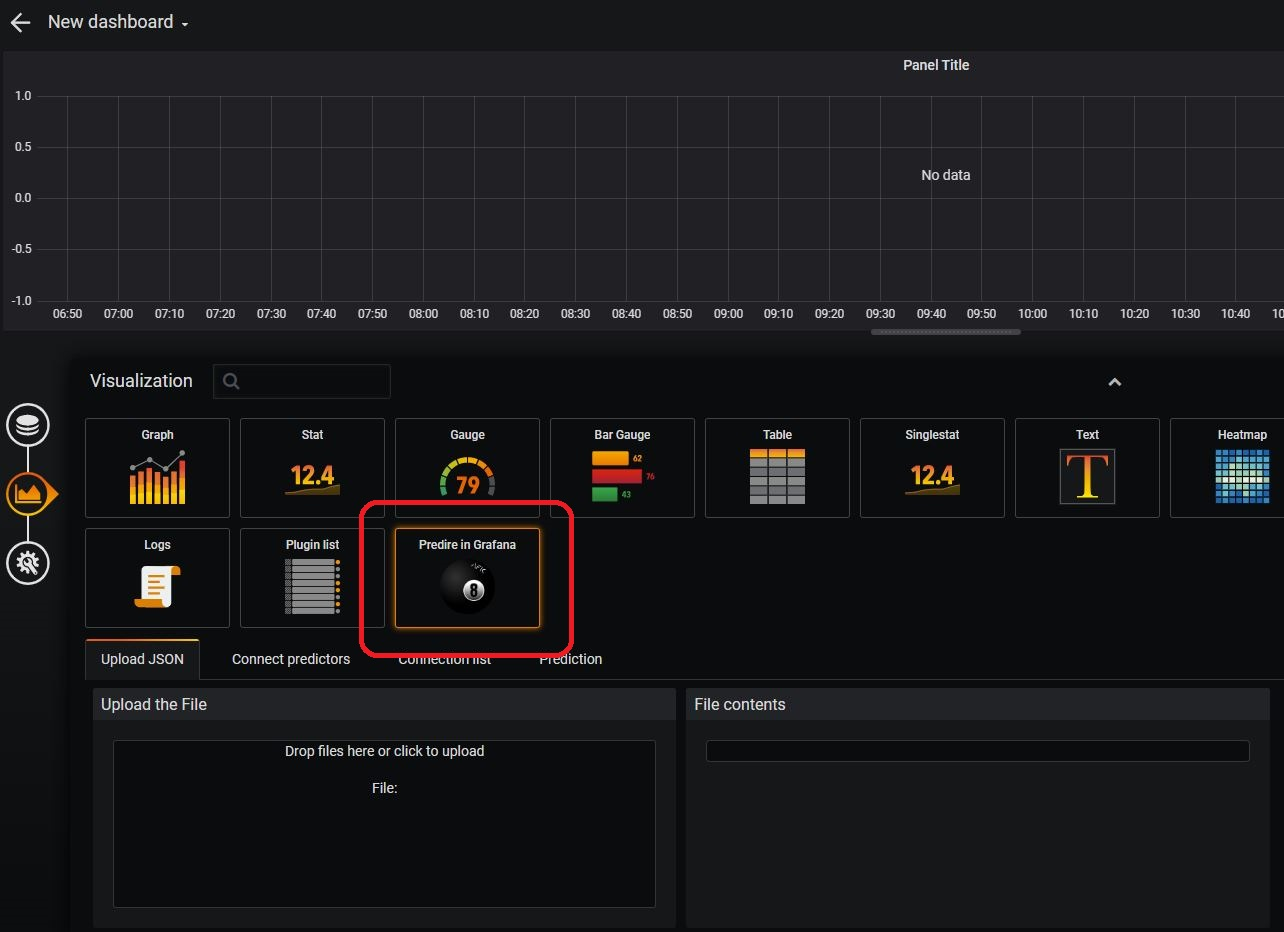
\includegraphics[scale=0.55]{img/plug-in/plugin_1.JPG}
\caption{"Predire in Grafana" Panel}
\end{figure}

\end{enumerate}

	
\subsection{Loading a JSON file}
The user can select the “Upload the file” button contained in the “Upload JSON” section.
This will open a window from which the JSON file can be selected.
Alternatively, the user can drag and drop the JSON file in the "Upload the file" section.
The content of the JSON file will be displayed in a panel called "File contents" to the right of the previously mentioned section.

\begin{figure}[H]
\centering
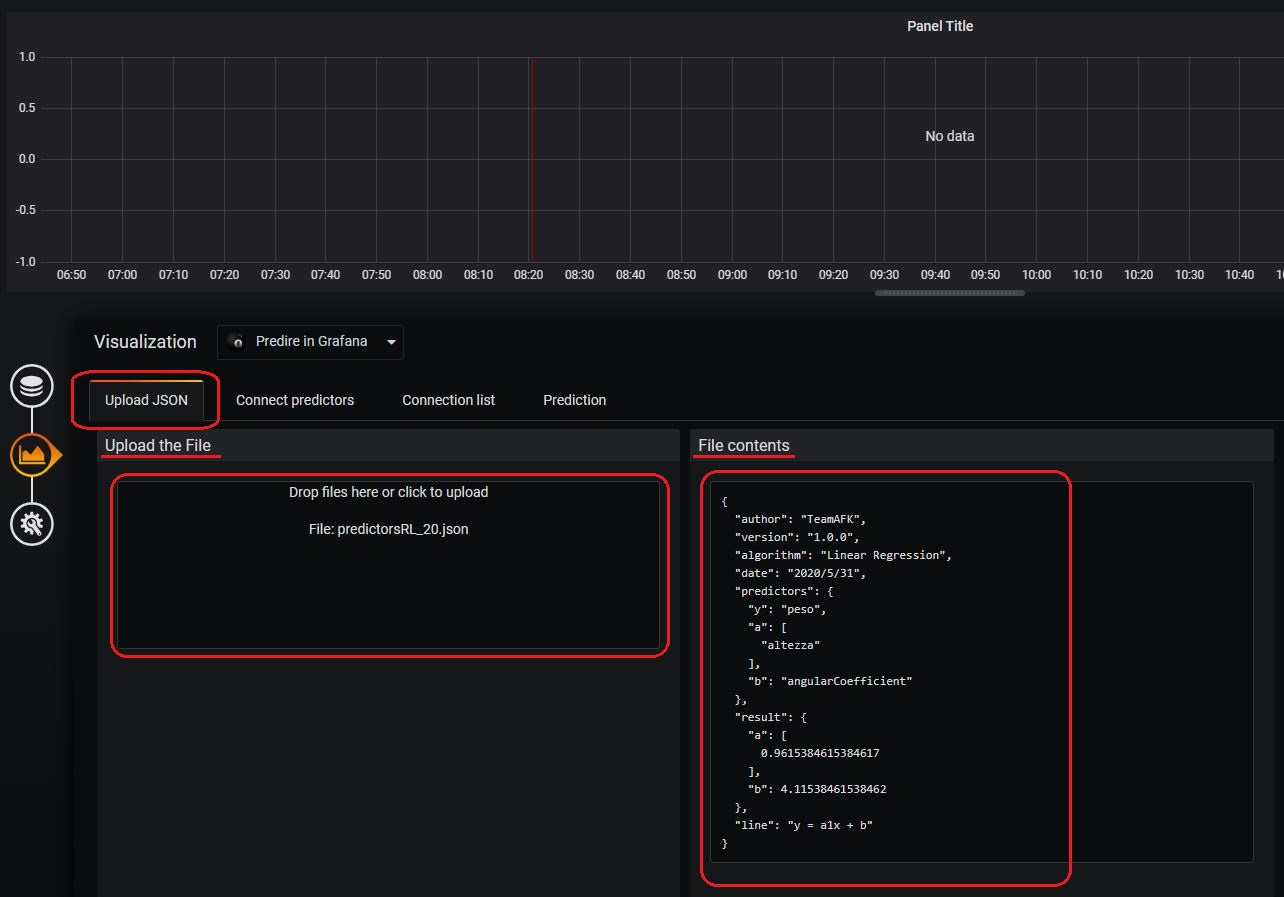
\includegraphics[scale=0.60]{img/plug-in/plugin_2.JPG}
\caption{Loading window and displayed loaded JSON}
\end{figure}


\subsection{Connecting predictors}
The portion of the software dedicated to the connection of the nodes can be accessed by selecting the "Connect predictors" tab:
\begin{enumerate}
	\item the user can choose from the “Insert connection” section which queries are to be associated with which nodes.
	Once all the nodes are connected, the user can select the "Add connection" button and confirm the operation;
	
\begin{figure}[H]
\centering
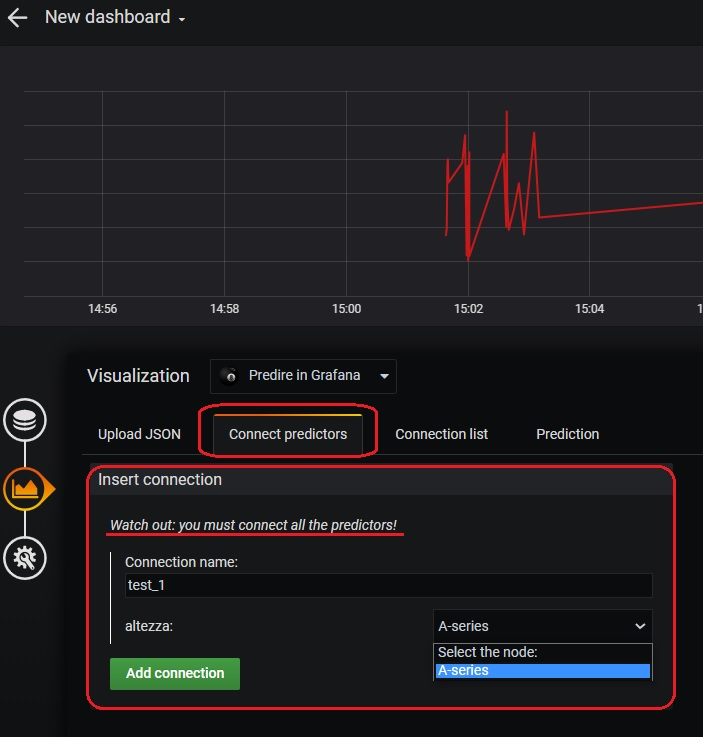
\includegraphics[scale=0.75]{img/plug-in/plugin_3.JPG}
\caption{Connection coupling (a)}
\end{figure}



\begin{enumerate}
\item should the user have not filled all the required fields, an error message will be displayed on selection of the "Add connection" button;

	
\begin{figure}[H]
\centering

\includegraphics[scale=0.60]{img/plug-in/plugin_4.JPG}
\caption{Connection coupling error message}
\end{figure}

\item once all the required fields are correctly chosen, a confirm message will be displayed. 

\begin{figure}[H]
\centering

\includegraphics[scale=0.60]{img/plug-in/plugin_5.JPG}
\caption{Connection coupling confirm message}
\end{figure}

\end{enumerate} 


\end{enumerate}



\subsection{Modifying the connections}
In this section the user can view all the predictor-data stream connections that have been made. This section can be accessed by selecting the "Connection list" tab.
The user can also modify the connection, by pressing on the "Edit" button, or delete it, by selecting the "Disconnect" button.

\begin{figure}[H]
\centering
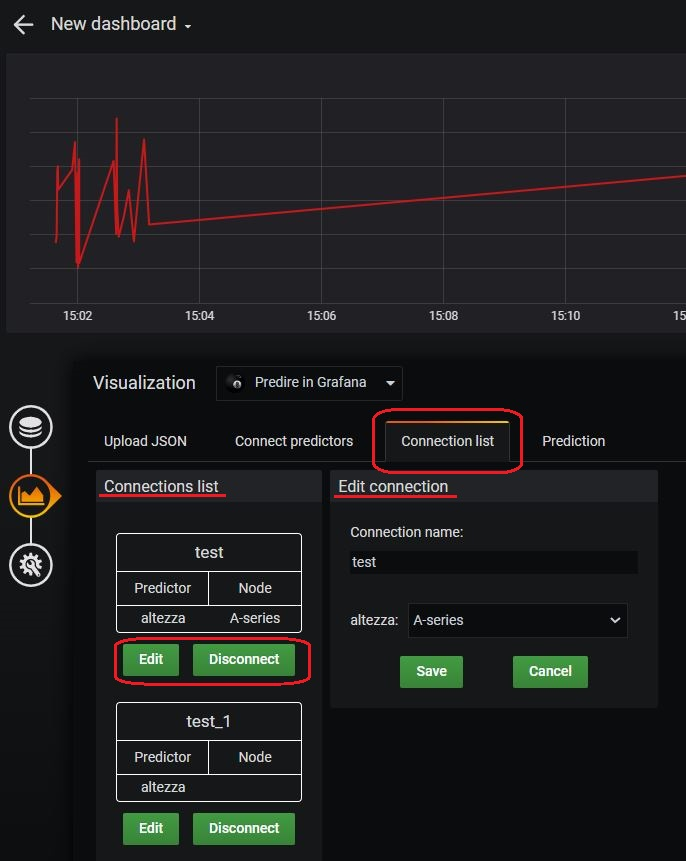
\includegraphics[scale=0.75]{img/plug-in/plugin_6.JPG}
\caption{Node linking}
\end{figure}


\subsection{Prediction operations}
In this last section the user will be able to launch the prediction algorithms of the plug-in. This section is accessed by selecting the "Prediction" tab. Here the user will be able to select, in the top right corner, a temporal policy by choosing starting and ending dates and choosing how often to sample the data. The user  also has access to two buttons, one called "Start monitoring", which starts the prediction operations, and a second one named "Enable saving", which saves the data collected up to the point it is pressed.\\

\begin{figure}[H]
\centering
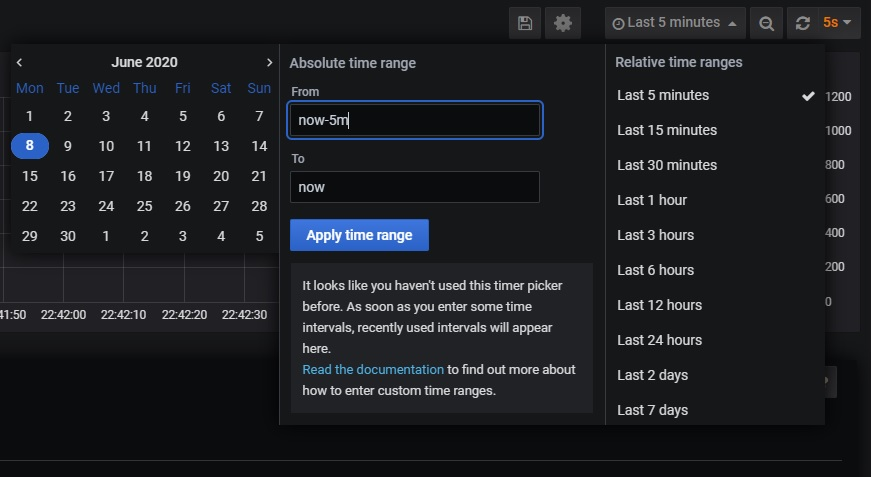
\includegraphics[scale=0.70]{img/plug-in/time_selector.png}
\caption{Time picker}
\end{figure}

When the prediction has been started, the "Start monitoring" button becomes "Stop monitoring", which, if pressed, will stop the monitoring.

\begin{figure}[H]
\centering
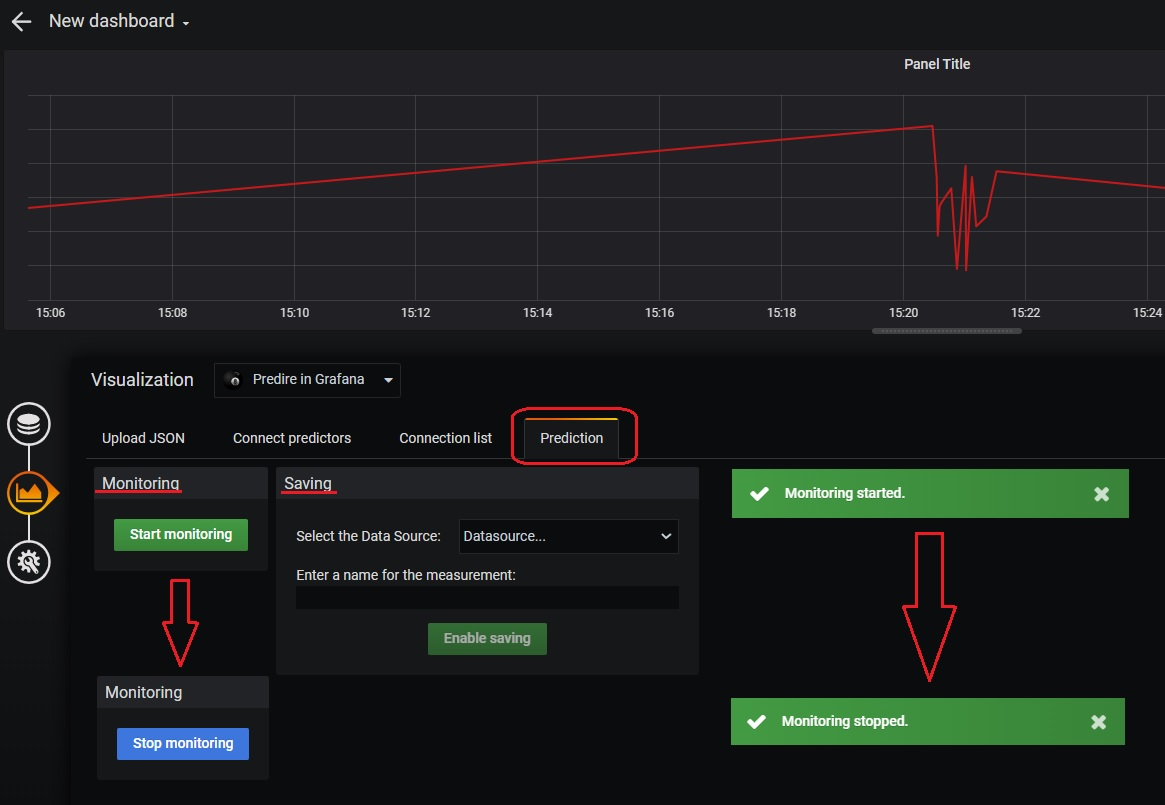
\includegraphics[scale=0.65]{img/plug-in/plugin_7.JPG}
\caption{Begin\textbackslash end data monitoring and Prediction save}

\end{figure} 
 


\pagebreak
\section{File structure}
	\subsection{JSON file structure}
JSON files which contain trained algorithm definition must be structured as it follow.	

		\subsubsection{Linear Regression}
		\begin{itemize}
			\item\textbf{author}: the file's author. Set in defaul as "TeamAFK";
			\item\textbf{version}: the training tool application version. Set in deafult as "1.0.0";
			\item\textbf{algorithm}: the trained algorithm . Set in default as "Linear Regression"; 	
			\item\textbf{date}: the current date when file is created;
			\item\textbf{predictors}: list of all predictors' labels. These labels are taken from CSV files.
			\item\textbf{result}: list of obtained coefficients from the training. In detail:
			\begin{itemize}
					\item\textbf{a}: list of coefficients values of the regression line formula;
					\item\textbf{b}: bias of the regression line formula;
				\end{itemize}
			\item\textbf{line}: regression line formula;
					
		\end{itemize}
		
		\begin{figure}[H]
		\centering
		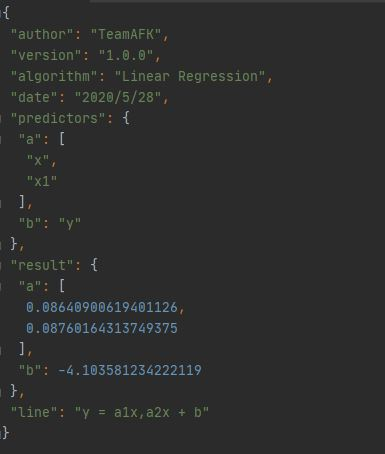
\includegraphics[scale=0.70]{../Developer_manual/img/linear_regression_json.jpg}
		\caption{Example of Linear Regression JSON file}
	\end{figure}	
	
		\subsubsection{Support Vector Machine}
		\subsubsection{Linear Regression}
		\begin{itemize}
			\item\textbf{author}: the file's author. Set in defaul as "TeamAFK";
			\item\textbf{version}: the training tool application version. Set in deafult as "1.0.0";
			\item\textbf{algorithm}: the trained algorithm . Set in default as "SVM"; 	
			\item\textbf{date}: the current date when file is created;
			\item\textbf{predictors}: list of all predictors' labels. These labels are taken from CSV files.
			\item\textbf{result}: list of obtained coefficients from the training. In detail:
				\begin{itemize}
					\item\textbf{a}: list of weights values of the regression line formula;
					\item\textbf{b}: bias of the regression line formula;
				\end{itemize}
			\item\textbf{line}: separation line formula.
					
		\end{itemize}
		
		\begin{figure}[H]
		\centering
		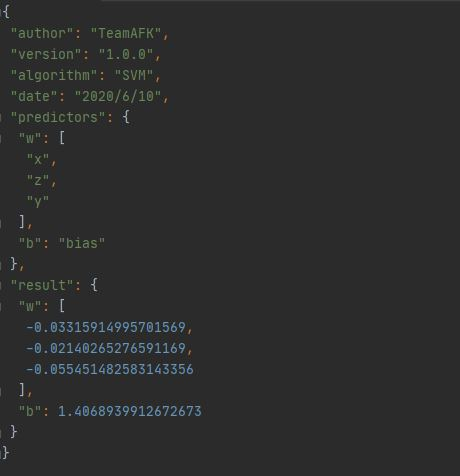
\includegraphics[scale=0.70]{../Developer_manual/img/support_vector_machine_json.jpg}
		\caption{Example of Linear Regression JSON file}
	\end{figure}	
		
	
	\subsection{CSV file structure}
Weather you use choose to train one algorithm intead of another one CSV file has a common structure:
	\begin{itemize}
		\item\textbf{first columns till y column}: each column represents a predictor;
		\item\textbf{y}: this column contains the results.	
	\end{itemize}	 

First line of CSV files must contain predictors tags while the other lines contain values. If you want to add a predictor you must insert a column, before y column, with the predictor tag as first line.

\begin{figure}[H]
		\centering
		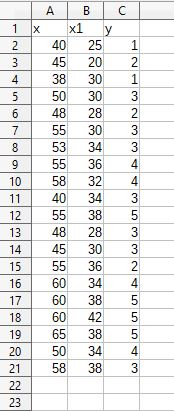
\includegraphics[scale=0.70]{../Developer_manual/img/linear_regression_csv.jpg}
		\caption{Example of Linear Regression CSV file}
	\end{figure}

In SVM CSV files you can find one more column named "label" which contains the data group. 

\begin{figure}[H]
		\centering
		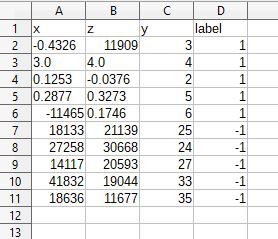
\includegraphics[scale=0.70]{../Developer_manual/img/support_vector_machine_csv.jpg}
		\caption{Example of Linear Regression CSV file}
	\end{figure}
 




\pagebreak
\section{Reporting Errors}
Should anomalies or errors encountered during the execution of the plug-in or the training tool, it is possibile to report them ad the follwing mail address: \href{mailto:gruppoafk15@gmail.com}{gruppoafk15@gmail.com}.

\subsection{Reporting Training Tool errors}
In the object field the type of error must be stated in the following way: [Error][Training tool],
the body of the mail must contain the  following statements:

\begin{itemize}
	\item operating system version;
	\item training tool version;
	\item detailed explanation of the encountered. error
\end{itemize}

\begin{figure}[H]
\centering

\includegraphics[scale=0.85]{img/mail/tool_mail.jpg}
\caption{Taining tool error mail template}
\end{figure}

\subsection{Reporting Plug-in errors}
To report Plug-in errors instead: the object field has to be compiled as such: [Error][Plug-in] and the body must contain the following statements:
\begin{itemize}
\item Grafana version;
\item plug-in version;
\item browser version;
\item operating system version;
\item  detailed explanation of the encountered.
\end{itemize}

\begin{figure}[H]
\centering
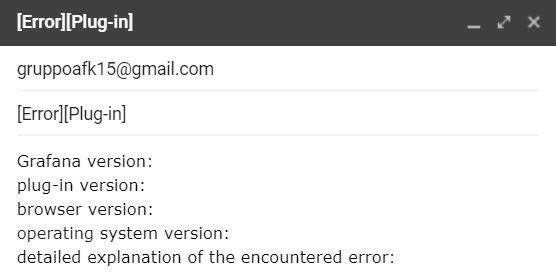
\includegraphics[scale=0.85]{img/mail/plug-in_mail.jpg}
\caption{Plug-in error mail template}
\end{figure}
\pagebreak

\appendix
\section{Glossary}

{\Large\textbf{A}\par}
\textbf{Application Logic}\\
Application Logic is any logic that is specific to some application

{\Large\textbf{B}\par}
\textbf{Business Logic}\\
It is the processing logic, in the form of source code, which manages the communication between a user interface and a database. It therefore contains the information that defines or they bind the way a company operates.

{\Large\textbf{C}\par}
\textbf{CSV}\\
CSV (comma-separated values) is a simple file format used to store tabular data, such as a spreadsheet or database.

{\Large\textbf{D}\par}
\textbf{DOM}\\
The Document Object Model (DOM) is a platform and language-neutral interface that allows programs and scripts to dynamically access and update the content, structure, and style of a document.

{\Large\textbf{L}\par}
\textbf{Linear Regression (LR)}\\
Linear regression (LR) is a linear approach to modeling the relationship between a scalar response (or dependent variable) and one or more explanatory variables (or independent variables). The case of one explanatory variable is called simple linear regression.

{\Large\textbf{G}\par}
\textbf{Grafana}\\
Grafana is a multi-platform open source analytics and interactive visualization web application. It provides charts, graphs, and alerts for the web when connected to supported data sources. It is expandable through a plug-in system. End users can create complex monitoring dashboards using interactive query builders.

\textbf{GUI}\\
A graphical user interface (GUI) is an interface through which a user interacts with electronic devices such as computers, hand-held devices and other appliances. 

{\Large\textbf{J}\par}
\textbf{JavaScript}\\
JS is a programming language that conforms to the ECMAScript specification. JavaScript is high-level, often just-in-time compiled, and multi-paradigm. 

\textbf{JSON}\\
JSON (JavaScript Object Notation) is a lightweight data-interchange format. It is easy for machines to parse and generate.

\textbf{JSX}\\
JSX is an extension of the JavaScript language based on ES6, and is translated into regular JavaScript at runtime.

{\Large\textbf{M}\par}
\textbf{Machine learning}\\
Machine learning (ML) is the study of computer algorithms that improve automatically through experience. Machine learning algorithms, such as LR or SVM, build a mathematical model based on sample data, known as "training data", in order to make predictions or decisions without being explicitly programmed to do so.

{\Large\textbf{N}\par}
\textbf{Node.js}\\
Node.js is an open-source, cross-platform, JavaScript runtime environment that executes JavaScript code outside a web browser. Node.js lets developers use JavaScript to write command line tools and for server-side scripts to produce dynamic web page content before the page is sent to the user's web browser.

\textbf{NPM}\\
NPM (Node Package Manager) is a package manager for the JavaScript programming language. It is the default package manager for the JavaScript runtime environment Node.js.

{\Large\textbf{O}\par}
\textbf{OS}\\
An Operating System (OS) is an interface between a computer user and computer hardware. An operating system is a software which performs all the basic tasks like file management, memory management, process management, handling input and output, and controlling peripheral devices.

{\Large\textbf{P}\par}
\textbf{Package}\\
A package (java package) is used to group related classes. They are used to avoid name conflicts, and to write a better maintainable code. 

\textbf{Presentation Logic}\\
The presentation logic of an application is where occurs almost of all interactions with the end user. Manages the reception of user inputs and the presentation of the output of the application to the latter.

{\Large\textbf{R}\par}
\textbf{React}\\
React is a JavaScript library for building user interfaces.

{\Large\textbf{S}\par}
\textbf{Support Vector Machine (SVM)}\\
In machine learning, Support Vector Machines (SVM) are supervised learning models with associated learning algorithms that analyze data used for classification and regression analysis.

{\Large\textbf{T}\par}
\textbf{Typescript}\\
TypeScript is a typed superset of JavaScript that compiles to plain JavaScript.



\end{document}